%!TEX root = ../main.tex

\chapter{Aufbau}
\label{ch:aufbau}

\section{Architektur}
\begin{figure}[ht]
    \centering
    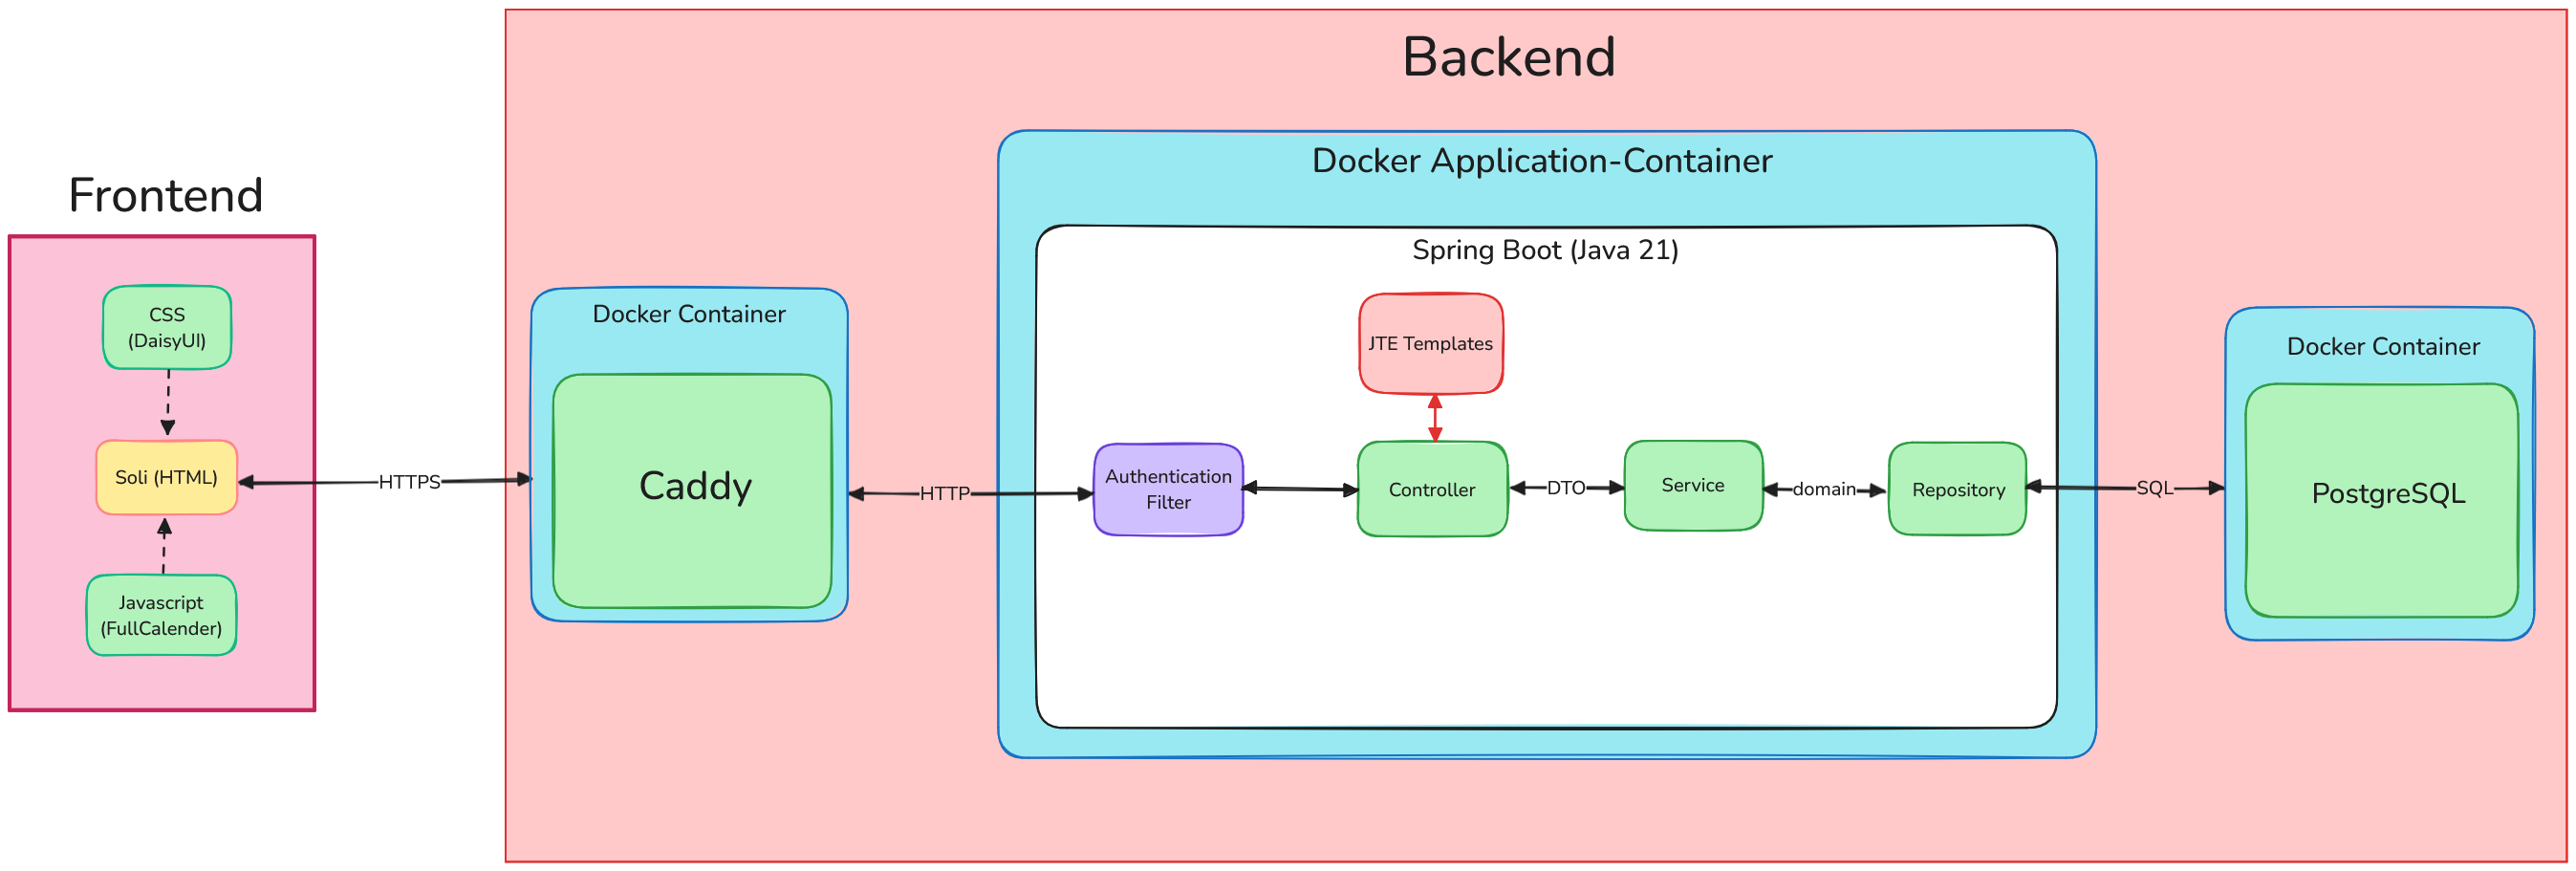
\includegraphics[width=\textwidth]{figures/architecture}
    \label{fig:architekturmodell}
\end{figure}
Die Architektur ist in \textbf{Frontend} und \textbf{Backend} unterteilt und folgt der \textbf{MVC-Struktur} zur klaren Trennung der Verantwortlichkeitsbereiche.
Das \textbf{Frontend} nutzt \textbf{HTML (Soli)}, \textbf{DaisyUI} für das Design und \textbf{FullCalendar} in JavaScript für die Kalenderfunktionalität.
Die Kommunikation mit dem Backend erfolgt sicher über \textbf{HTTPS}.

Ein \textbf{Caddy-Server}, in einem Docker-Container, dient als HTTPS-Reverse-Proxy und leitet Anfragen an das Backend weiter.
Das \textbf{Backend} basiert auf \textbf{Spring Boot} (Java 21) und läuft in einem Docker-Container. Dort prüft ein \textbf{Authentication Filter} die Anfragen,
die von \textbf{Controllern} verarbeitet werden. Mithilfe von \textbf{JTE Templates} werden dynamische HTML-Antworten generiert.
Die \textbf{Businesslogik} liegt in den \textbf{Services}, die Anfragen koordinieren und weiterleiten.
Die \textbf{Repositories} kapseln den SQL-Zugriff und ermöglichen eine saubere, abstrahierte Kommunikation mit der \textbf{PostgreSQL-Datenbank} in einem separaten Container.

Dank \textbf{Server-Side Rendering} bietet die Architektur dynamische Inhalte und hohe Skalierbarkeit. Der Einsatz gängiger Technologien wie \textbf{Docker} sorgt für einfache Bereitstellung und Wartbarkeit.
\clearpage

\section{Klassendiagramm}
\begin{figure}[ht]
    \centering
    \includegraphics[width=0.62\textwidth]{figures/classes}
    \label{fig:klassendiagramm}
\end{figure}
\clearpage